\title{Computer Graphics Lab, Prof. Dr. Philipp Jenke}

\documentclass[a4letter,10pt]{scrartcl}
\usepackage{a4wide}

% deutsche Silbentrennung
\usepackage[ngerman]{babel}

% wegen deutschen Umlauten
\usepackage[applemac]{inputenc}

% Kein Einr�cken zu Beginn eines Absatzes
\setlength\parindent{0pt}

% Java listings
%\usepackage{listings}

%% Special tabular version
\usepackage{tabularx}

% ben�tigt zum Setzen der Fu�zeile
\usepackage{scrpage2}

% Ben�tigt, um auf LastPage zugreifen zu k�nnen
\usepackage{lastpage}

\usepackage{graphicx}
\usepackage{subfigure}

\pagestyle{scrheadings}    
\renewcommand*{\headfont}{\normalfont}

% Setzen der Kopfzeile
\setlength{\headheight}{2.5cm}
\clearscrheadfoot
\chead{Computergrafik Framework - Architekturdokumentation, Komponenten und Konzepte}

\begin{document}

%-------------- Titel -------------

\begin{titlepage}
\author{Philipp Jenke\\Hochschule f�r Angewandte Wissenschaften (HAW), Hamburg} 
\title{Computergrafik Framework  - Architekturdokumentation, Komponenten und Konzepte} 
\date{\today} 
\maketitle
\end{titlepage}

\tableofcontents
\newpage

\section{Einleitung}

Ziel dieses Dokumentes ist es, die grundlegenden Konzepte und die architektonischen Entscheidungen f�r die Softwarekomponenten in der Software-Bibliothek darzulegen. Au�erdem werden Installationsanleitungen zum Auschecken und f�r die Inbetriebnahme der Projekte gegeben. 

\section{Getting Started}
\label{section:cg}

Wir beginnen mit dem Schnelleinstieg. 

\subsection{Voraussetzungen}

Zun�chst m�ssen auf dem Rechner die Voraussetzungen sichergestellt werden:
\begin{itemize}
\item Oracle Java 1.8 oder neuer \\ (\emph{http://www.oracle.com/technetwork/java/javase/overview/index.html})
\item Gradle 2.6 oder neuer (\emph{https://gradle.org/})
\item Git 2.3 oder neuer (unterschiedliche Quellen je nach OS)
\item Entwicklungsumgebubng
	\begin{itemize} 
	\item (entweder) Eclipse 4.5 (Mars) oder neuer (\emph{https://eclipse.org/})
	\item (oder) Intellij IDEA 14.X ((\emph{https://www.jetbrains.com/idea/})
	\end{itemize}
\end{itemize}

\subsection{Repository Auschecken [nicht notwendig bei Verwendung von IntelliJ]}

Das Repository mit allen notwendigen Sourcen und sonstigen Dateien finden sich unter folgender URL: \\
\emph{git.informatik.haw-hamburg.de/srv/git/computergrafik/computergraphics}.\\

\begin{itemize}
	\item Es muss auf den Entwicklungsrechner gecloned werden:\\
	\verb+git clone ssh://<login>@git.informatik.haw-hamburg.de/+\\
	\verb+     srv/git/computergrafik/computergraphics+
	\item \textbf{Kompilieren mit Gradle:} Gradle bietet die M�glichkeit, das Projekt �ber die Kommandozeile zu kompilieren. Dazu muss im Projektverzeichnis (Elternverzeichnis der Unterprojekte wie \emph{graphics\_core}) folgender Befehl ausgef�hrt werden:\\
	\verb+gradle build+
\end{itemize}

\subsection{Entwicklungsumgebung}

Im Prinzip kann man mit jeder beliebigen Entwicklungsumgebung (oder einem Text-Editor) arbeiten. Anleitungen werden hier f�r Eclipse und IntelliJ gegeben.

\subsubsection{Eclipse}

\begin{itemize}
	\item \textbf{Projekte erstellen:} Zum Erstellen der Eclipse-Projektdateien wird wieder Gradle verwendet:\\
	\verb+gradle eclipse+\\
	Nach erfolgreicher Ausf�hrung dieses Befehls befinden sich Eclipse-Projektdateien (\emph{.project}, ...) in jedem der Unterprojekte.
	\item \textbf{Import:} Je nachdem, was genau gemacht werden soll, ben�tigt man verschiedene Unterprojekte. Beispielhaft soll hier die Demo-Anwendung \verb+ObjTriangleMesh+ ausgef�hrt werden. Diese befinden sich in dem Unterprojekt \emph{apps}. Um das Projekt in Eclipse zu importieren sind die folgenden Schritte notwendig:
	\begin{itemize}
		\item File
		\item Import
		\item Existing Projects into Workspace
		\item Select root directory: $<$\emph{Hier muss das Unterverzeichnis \emph{apps} ausgew�hlt werden}$>$
		\item Finish
	\end{itemize}
	Nun ist das Projekt in Eclipse importiert und erscheint im Projekt-Exporer. 
\end{itemize}

\subsubsection{IntelliJ}

\begin{itemize}
\item \textbf{Intellij konfigurieren}, so dass es den nativen SSH-Client benutzt (openSSH unter Linux Mint). Der schon in Intellij eingebaute SSH-Client hat mit dem Git-Server der HAW bei mir nicht funktioniert.)
Configure $\rightarrow$ Settings $\rightarrow$ Version Control $\rightarrow$ Git $\rightarrow$ SSH executable build-in auf native �ndern.
\item \textbf{Auschecken des Repositories:} Check out from Version Control $\rightarrow$ Git\\
Git Repository URL:\\
\verb+ ssh://<login>@git.informatik.haw-hamburg.de/+\\
\verb+     srv/git/computergrafik/computergraphics+\\
Parent Directory: Standardgem��:\\ 
\verb+/home/<account>/IdeaProjects+\\
oder\\ 
\verb+C:\Users\<account>\IdeaProjects+\\
Directory Name: \verb+computergraphics+. Anschlie�end clonen.
\item \textbf{Importieren des Projektes mit Gradle:} Nach dem clonen fragt Intellij, ob die \emph{gradle.build} Datei ge�ffnet werden soll. Dies best�tigen wir mit Ja. Ist Gradle auf dem Rechner installiert muss man hier lediglich den Pfad angeben. Ansonsten bietet Intellij die Option einen \emph{Customizable Gradle Wrapper} zu benutzen. Im zweiten Fall ist die Installation von Gradle nicht notwendig.

\end{itemize}

\subsection{Abschluss}

\begin{itemize}
	\item \textbf{Asset-Pfad einrichten:} Viele Programme verwenden Daten (z.B. Icons oder Dreiecksnetze). Standarddaten finden sich im Projektverzeichnis im Unterverzeichnis \emph{assets}. Damit ausgef�hrte Programme diese Assets auch finden, muss der Pfad zu diesem Verzeichnis bekannt gegeben werde. Dazu wird der absolute Pfad des Unterverzeichnisses \emph{assets} in der Textdatei \emph{resources.txt} eingetragen.
	\item \textbf{Demo-Programm starten:} Im Package \verb+cgresearch.apps.trianglemeshes+ kann nun die Klasse \verb+ObjTriangleMesh+ durch \emph{Rechtsklick} $\rightarrow$ \emph{Run As} $\rightarrow$ \emph{Java Application} ausgef�hrt werden. Hat alles geklappt, dann �ffnet sich ein Fenster und ein 3D-Modell erscheint.
\end{itemize}

%\subsubsection{libGDX}
%
%Zun�chst muss die Entwicklungsumgebung f�r die Verwendung von libGDX angepasst werden. In dieser Anleitung wird zun�chst davon ausgegangen, dass die Anwendung f�r Desktop (egal welches Betriebssystem) und f�r Android Mobil verwendet werden soll. Au�erdem wird davon ausgegangen, dass Eclipse als Entwicklungsumgebung verwendet wird. Zum Einrichten folgt man am Besten der Anleitung zur Einrichtung von libGDX\footnote{http://libgdx.badlogicgames.com/documentation.html}. Prinzipiell m�ssen folgende Komponenten eingerichtet werden:
%\begin{itemize}
%\item JDK 7+
%\item Android SDK
%\item Eclipse Plugin zur Android-Entwicklung
%\item Eclipse Plugin zur Verwendung von Grade (wird f�r das Setup von libGDX ben�tigt)
%\end{itemize} 
%
%Dann wird das zugeh�rige Repository gecloned. Das Repository findet sich unter folgender URL: \emph{git.informatik.haw-hamburg.de/srv/git/computergrafik/cg\_libgdx}.
%
%Schliesslich wird das Projekt in Eclipse importiert. Dazu w�hlt man
%\begin{itemize}
%\item File
%\item Import
%\item Gradle
%\item Gradle Project
%\item Verzeichnis mit dem Repository ausw�hlen
%\item Build Model
%\end{itemize}
%
%In Eclipse werden damit mehrere neue Projekte eingerichtet, wir betrachten hier zun�chst nur 
%\begin{itemize}
%\item \textbf{cg\_libgdx-core:} Hier ist die Anbindung zwischen dem cgresearch Framework und libGDX umgesetzt. Dieses Package muss nur ver�ndert werden, wenn die Anbindung erweitert werden soll, z.B. wenn man eine neue RenderObjectFactory f�r libGDX hinzuf�gen will.
%\item \textbf{cg\_libgdx-desktop:} Dies ist das Startprojekt f�r Desktop-Anwendungen. Um eine Anwendung mit libGDX zu starten, muss man diese in der Klasse \verb+DesktopLauncher+ in den Konstruktor von LibGdxFrame als Parameter stecken. Dann kann man die Anwendung mit libGdx-Rendering auf dem Desktop starten.
%\item \textbf{cg\_libgdx-android:} Dies ist das Startprojekt f�r Android-Anwendungen. Um eine Anwendung mit libGDX zu starten, muss man diese in der Klasse \verb+AndroidLauncher+ in den Konstruktor von LibGdxFrame als Parameter stecken. Dann kann man die Anwendung mit libGdx-Rendering auf dem Desktop starten.
%\end{itemize}
%
%Damit die libGDX-Projekte die Funktionalit�t aus dem cgresearch Framework kennen, muss dieses in Form eines .jars inkludiert werden. Dazu geht man folgendermassen vor:
%
%\begin{itemize}
%\item \textbf{Erzeugen des Jars:} Um aus dem cgresearch Framework ein Har-Archiv zu erzeugen starten man in der Kommandozeile nacheinander die folgenden zwei Befehlen (setzen Maven voraus!):
%\begin{itemize}
%\item \verb+mvn clean+
%\item \verb+mvn package+
%\end{itemize}
%Das erzeugte Jar mit dem Namen cgreasearch.jar findet man dann im Unterverzeichnis \emph{target}
%\item \textbf{Jar in das libGdx-Projekt bewegen:} Die Jar-Datei muss an in das libGdx Projekt bewegt werden. Es soll in folgedem Verzeichnis liegen: \emph{core/build/libs}.
%\item \textbf{Bibliothek in Projekte einf�gen} Zuletzt muss das Jar als externe Bibliothek in alle drei libGdx-Projekte integriert werden. Das geschieht �ber \emph{Rechtsklick auf das Projekt} $\rightarrow$ \emph{Properties} $\rightarrow$ \emph{Java Build Path} $\rightarrow$  \emph{Libraries} $\rightarrow$  \emph{Add External Jar}. 
%\end{itemize}
%
%\textbf{Resourcen/Assets} Ressourcen und Assets, die unter libGdx verwendet werden sollen m�ssen auch im \emph{assets}-Ordner libGdx-Projekt liegen. Der \emph{assets}-Ordner liegt im Unterordner \emph{android}. F�r den Zugriff aus dem Desktop-Projekt muss der Ordner entweder kopiert werten oder es muss ein Symbolischer Link (\emph{ln -s}) erzeugt werden. Au�erdem muss man in der Resourcen-Konfigurationsdatei \emph{resources.ini} den Pfad je nach Betriebssystem anpassen (siehe Abschnitt \ref{section:ressourcen}).
%
\section{Komponenten}
\label{section:cganwendung}

\subsection{Module}

Das Framework besteht aus folgenden Modulen

\begin{itemize}
\item \textbf{graphics\_core:} Szenengraph (siehe Abschnitt \ref{sec:scene_graph}), Interfaces f�r die Bausteine (Anwendung, UI und Rendering), Picking-Funktionalit�t, Kamera, Datenstrukturen und Algorithmen, I/O, Material
\item \textbf{rendering\_jogl:} Rendering mit OpenGL (hier JOGL)
\item \textbf{apps:} Programme, die die Grafik-Funktionalit�t verwenden 
\item \textbf{electronics:} Schnittstellen zu verschiedenen Elektronik-Komponenten wie Sensoren und Aktoren
\item \textbf{smart\_home\_apps:} Programme aus Smart Home-Bereich
\item \textbf{rc\_vehicles:} Zwei RaspberryPi-basierte Steuerungsprogramm (Boot, Bot)
\item \textbf{smart\_home\_visualization:} Visualisierungsl�sungen f�r das Smart Home (Kombination aus Smart Home und Grafik)
\end{itemize}

Die Abh�ngigkeiten zwischen den Teilprojekten sind in Abbildung \ref{fig:abhaengigkeiten_projekte} aufgezeigt.

\begin{figure}[ht]
\centering
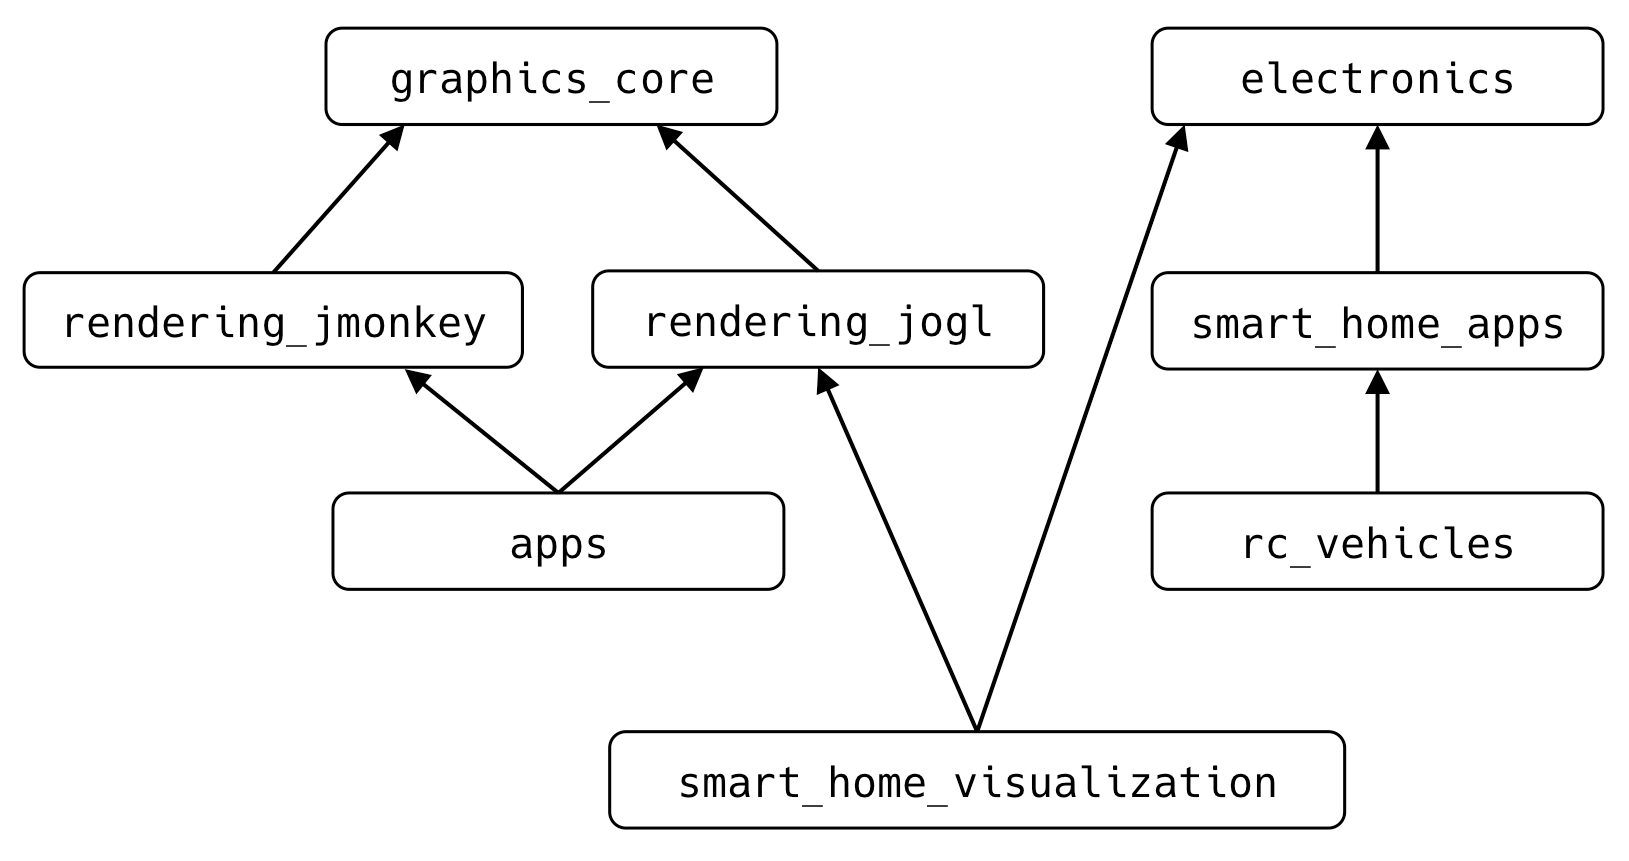
\includegraphics[height=5cm]{images/abhaengigkeiten_projekte.png}
\caption{Abh�ngigkeiten zwischen den Teilprojekten}
\label{fig:abhaengigkeiten_projekte}
\end{figure} 

Im Projektverzeichnis befinden sich au�erdem die folgenden Unterverzeichnisse, die keinen Code beinhalten:

\begin{itemize}
\item \textbf{assets:} Daten f�r die Anwendungen wie Icons und Dreiecksnetze
\item \textbf{doc:} Dokumentation f�r das Framework, u.a. dieses Dokument
\item \textbf{doc:} Skripte zum Verwenden des Frameworks auf einem Raspberry Pi
\end{itemize}

\begin{figure}[ht]
\centering
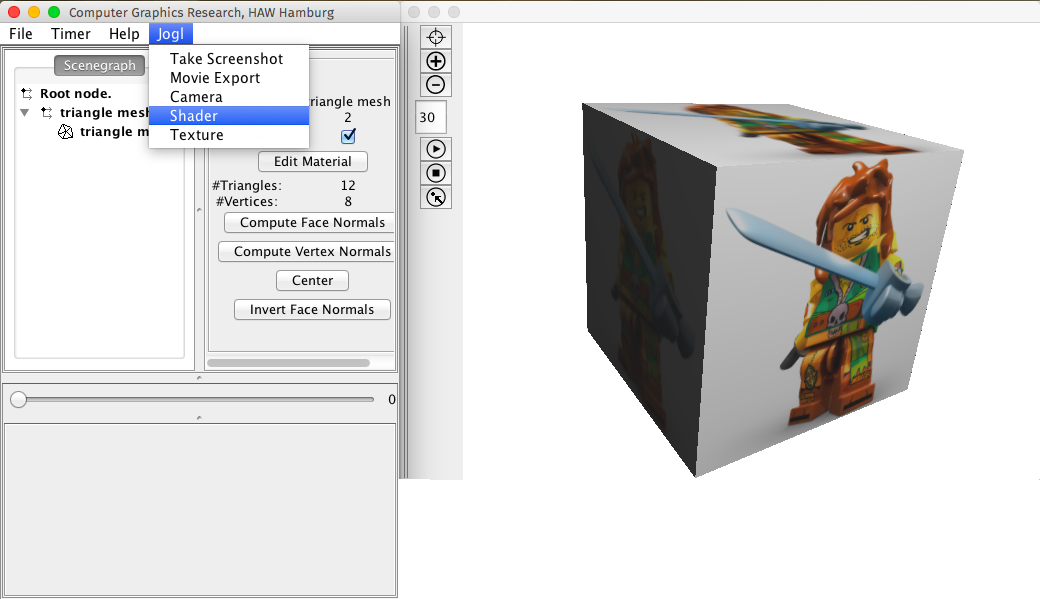
\includegraphics[height=8cm]{images/cgresearch.png}
\caption{Screenshot einer Anwendung mit dem cgresearch Framework. Das Fenster besteht aus verschiedenen Bl�cken: 3D-View (rechts), Debug-Konsole (unten), Szenengraph und Controller (oben links) Editor-Dialoge (Mitte) und Men�.}
\label{fig:cgapplication.png}
\end{figure} 

\subsection{Anwendungsobjekt}

In diesem Abschnitt wird beschrieben, wie mit dem cgresearch Framework eine Anwendung geschrieben werden kann. Als Rendering-System wird JOGL (siehe Abschnitte \ref{section:JOGL}) verwendet. Die Anwendung liegt im Teilprojekt \emph{apps}.

Im Zentrum einer Anwendung steht ein \verb+CgApplication+-Objekt. Darin spielt sich die eigentliche Logik der Anwendung ab. Zur Darstellung wird (optional) eine Instanz eines Rendering-Frames erzeugt. Auch das Benutzerinterface ist eine optionale Komponente. Die Klasse \verb+JoglSwingUserInterface+ stellt beispielsweise ein Benutzerinterface f�r das JOGL-System mit Java Swing bereit.

Die main-Methode der Anwendung k�nnte also lauten:
\begin{verbatim}
new ConsoleLogger(Logger.VerboseMode.DEBUG);
ResourcesLocator.getInstance().parseIniFile("resources.ini");
CgApplication app = new TriangleMeshFrame();
new JoglFrame(app);
new JoglSwingUserInterface(app);
\end{verbatim}
Zu dem Logger finden Sie Informationen im Abschnitt \ref{sec:logging}, der \verb+ResoucesLocator+ ist in Abschnitt \ref{section:ressourcen} dargestellt.

\subsection{Rendering}

Aktuell steht prim�r ein System f�r das Rendering zur Verf�gung:
\begin{itemize}
\item \verb+JoglFrame+ (JOGL)
\end{itemize}

Die Rendering-Systeme werden ausf�hrlicher in Abschnitt \ref{sec:rendering} besprochen. Neben dem JOGL-System wird rudiment�r auch jMonkey als Render-Engine unterst�tzt.

\subsection{Grafische Benutzerschnittstelle}

Aktuell  stehen zwei Klassen (und damit Systeme) f�r das Benutzerinterface (UI) zur Verf�gung:
\begin{itemize}
\item \verb+SwingUserInterface+ (Java Swing)
\item \verb+JoglSwingUserInterface+ (Java Swing mit Zusatzfunktionalit�t f�r JOGL)
\end{itemize}

Die meisten Anwendungen werden durch ein grafisches Benutzerinterface (GUI) gesteuert. In einer Anwendung k�nnen Sie eigene Benutzerinterfaces umsetzen und registrieren. Diese tauchen dann als zus�tzlicher Tab im Fensterbereich \emph{Szenengraph und Controller} auf. Zum Schreiben eines solchen Controllers implementieren Sie eine eigene Klasse, die von der abstrakten Klasse \verb+IApplicationControllerGui+ erbt. Diese Klasse wiederum erbt von \verb+JPanel+. Sie m�ssen also das \verb+this+-Objekt mit Ihrem GUI bef�llen. Anschliessend registrieren Sie das Objekt bei Ihrer Instanz f�r die Grafische Benutzeroberf�che �ber die Methode \verb+registerApplicationGUI()+. Hier eine einfache Beispiel-Implementirerung f�r ein GUI, das aus einem Button besteht, der einen Tetraeder erzeugt:

\begin{verbatim}
public class PJController extends IApplicationControllerGui 
 	 	 	implements ActionListener {
 	public PJController() {
 	 	JButton button = new JButton("PJ!");
 	 	button.addActionListener(this);
 	 	add(button);
 	}

 	@Override
 	public String getName() {
 	 	return "PJ";
 	 }

 	@Override
 	public void actionPerformed(ActionEvent e) {
 	 	CgNode node = new CgNode(TriangleMeshFactory.createTetrahedron(), "Tetra");
 	 	getRootNode().addChild(node);
 	}
}
\end{verbatim}

\subsection{Men�s}

Ihre GUI-Anwendung kann auch um benutzerdefinierte Men�s erweitert werden. Das Vorgehen ist sehr �hnlich zum Vorgehen beim Erstellen einer eigenen GUI-Komponente aus dem vorherigen Abschnitt. Zun�chst muss eine Men�klasse implementiert werden, die von der abstrakten Klasse \verb+CgApplicationMenu+ abgeleitet ist. Diese Instanz registrieren Sie in Ihrer GUI-Instance: 
\begin{verbatim}
	registerApplicationMenu(new <Men�klasse>)); 
\end{verbatim}

Die Elternklasse der Men�klasse selber erbt von \verb+JMenu+. Daher m�ssen Sie einfach das \verb+this+-Objekt mit den gew�nschten Men�eintr�gen bef�llen, um ein Men� zu erstellen. Eine Beispielumsetzung einer Men�-Klasse ist:	

\begin{verbatim}
public class PjMenu extends CgApplicationMenu {
 	public MyMenu() {
 	 	super("MyMenu");
 	 	JMenuItem itemPrintMessage = new JMenuItem("Print message");
 	 	itemPrintMessage.addActionListener(new ActionListener() {
 	 	 	public void actionPerformed(ActionEvent e) {
 	 	 	 	System.out.println("Message");
 	 	 	}
 	 	});
 	 	add(itemPrintMessage);
 	}
}
\end{verbatim}


\subsection{Ressourcen}
\label{section:ressourcen}

An mehreren Stellen im cg-Framework wird auf Ressourcen aus dem Dateisystem zugegriffen (z.B. Icons, Bilder, Netze, Texturen, ...). Diese k�nnen sich in unterschiedlichen Pfaden befinden. Die Resourcenpfade werden zentral �ber eine Singleton-Klasse {\verb ResourcesLocator } verwaltet. In jedem Programm, das das Framework verwendet, muss daher der {\verb ResourcesLocator } mit den notwendigen Ressoucenpfaden gef�llt werden. Dazu stehen zwei Methoden zur Verf�gung: 

\begin{itemize}
	\item {\verb addPath(String) } Hinzuf�gen eines Pfades
	\item {\verb parseIniFile(String) } Lesen eine Liste von Pfaden (zeilenweise) aus einer INI-Datei
\end{itemize}

Alle Ressourcen, die intern geladen werden (z.B. Icons, Netze, Texturen), verwenden den {\verb ResourcesLocator }, um alle Resourcenpfade zu durchsuchen. Greift man in einem Anwendungsprogramm auch direkt auf Ressourcen zu, dann kann man die Methode {\verb getPathToResource(String) } verwenden. Diese liefert entweder einen g�ltigen Pfad f�r eine Resource oder null, falls die Ressource in keinem der Ressourcenpfade gefunden wurde.

Die Ressourcen, die direkt mit dem Projekt cgresearch bereitgestellt werden, befinden sich im Projektverzeichnis im Unterverzeichnis \emph{assets}.

\subsection{Logging}
\label{sec:logging}

Innerhalb des Frameworks wird ein konsistentes Logging-System verwendet. Der Logger ist als Singleton implementiert und kann folgendermassen erreicht werden:

\begin{verbatim}
Logger logger = Logger.getInstance();
\end{verbatim}

Dem Logger k�nnen folgende Nachrichten geschickt werden:

\begin{itemize}
\item \textbf{Nachricht:} Generelle Nachricht, wird normalerweise sofort ausgegeben
\item \textbf{Debug-Nachricht:} Debugging-Nachricht, wird normalerweise nur ausgegeben, wenn Debugging aktiviert ist
\item \textbf{Exception:} Auftritt einer Exception, wird normalerweise sofort ausgegeben.
\item \textbf{Error:} Auftritt eines Fehlers, wird normalerweise sofort ausgegeben.
\end{itemize}

Aktuell sind folgende Logger umgesetzt:

\begin{itemize}
\item \verb+ConsoleLogger+ Ausgabe auf der Konsole
\item \verb+LoggerPane+ Wird bei Verwendung der Swing-GUI angezeigt
\end{itemize}
\section{Konzepte}

\subsection{Vektoren und Matrizen}
\label{sec:math}

\begin{verbatim} 
cgresearch.core.math
\end{verbatim}

Um die Architektur m�glichst flexibel zu halten, werden auf Vektoren und Matrizen nur �ber Interfaces zugegriffen (\verb+IVector3, IVector4, IMatrix3, IMatrix4+). Im Package gibt es au�erdem eine Fabrik-Klasse (\verb+VectorMatrixFactory+) mit der Instanzen von Vektoren und Matrizen erzeugt werden k�nnen. Dazu gibt es Referenzimplementierungen f�r die Interfaces. Gegebenenfalls werden diese sp�ter noch durch performantere Implementierungen ersetzt.

\subsection{Szenengraph}
\label{sec:scene_graph}

\begin{verbatim} 
cgresearch.graphics.scenegraph
\end{verbatim}

\begin{figure}[ht]
\centering
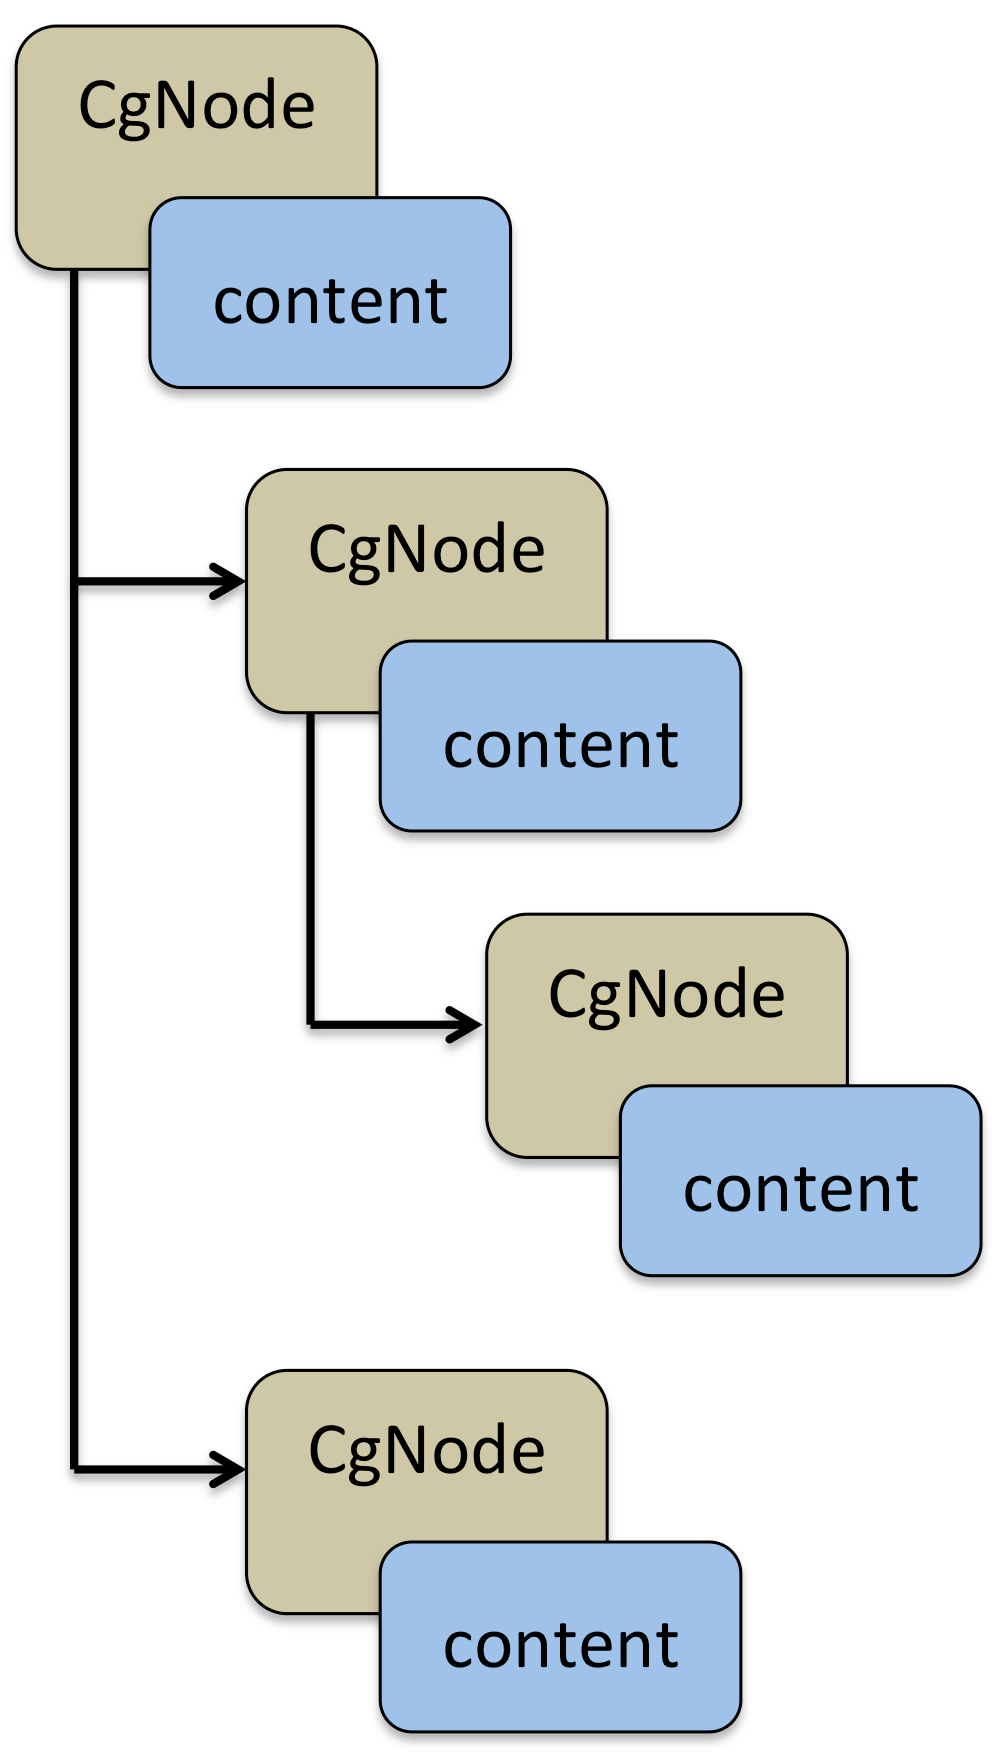
\includegraphics[height=6cm]{images/szenengraph.png}
\label{fig:szenengraph.png}
\caption{Der Szenengraph besteht aus Knoten vom Type CGNode. Jeder Knoten referenziert einen Inhalt (content). Dabei kann es sich z.B. um ein Dreiecksnetz (ITriangleMesh) handeln.}
\end{figure} 

Alle Daten werden in einem Szenengraph organisiert. Der Szenengraph besteht aus Knoten vom Type \verb+CgNode+. Ein Knoten kann unterschiedliche Daten repr�sentieren. Auf die Daten wird mit der Methode 
\begin{verbatim}
public ICgNodeContent getContent();
\end{verbatim}
zugegriffen.

\subsection{Rendering}
\label{sec:rendering}

\begin{verbatim} 
cgresearch.rendering
\end{verbatim}

Es werden unterschiedliche Rendering-Systeme unterst�tzt. Aktuell gibt es Implementierungen von JOGL (Abschnitt \ref{section:JOGL}) und jMonkey (Abschnitt \ref{section:jMonkey}). Nicht alle Implementierungen unterst�tzen die vollst�ndige Funktionalit�t. JOGL wird aktuell prim�r weiterentwickelt.

\begin{figure}[ht]
\centering
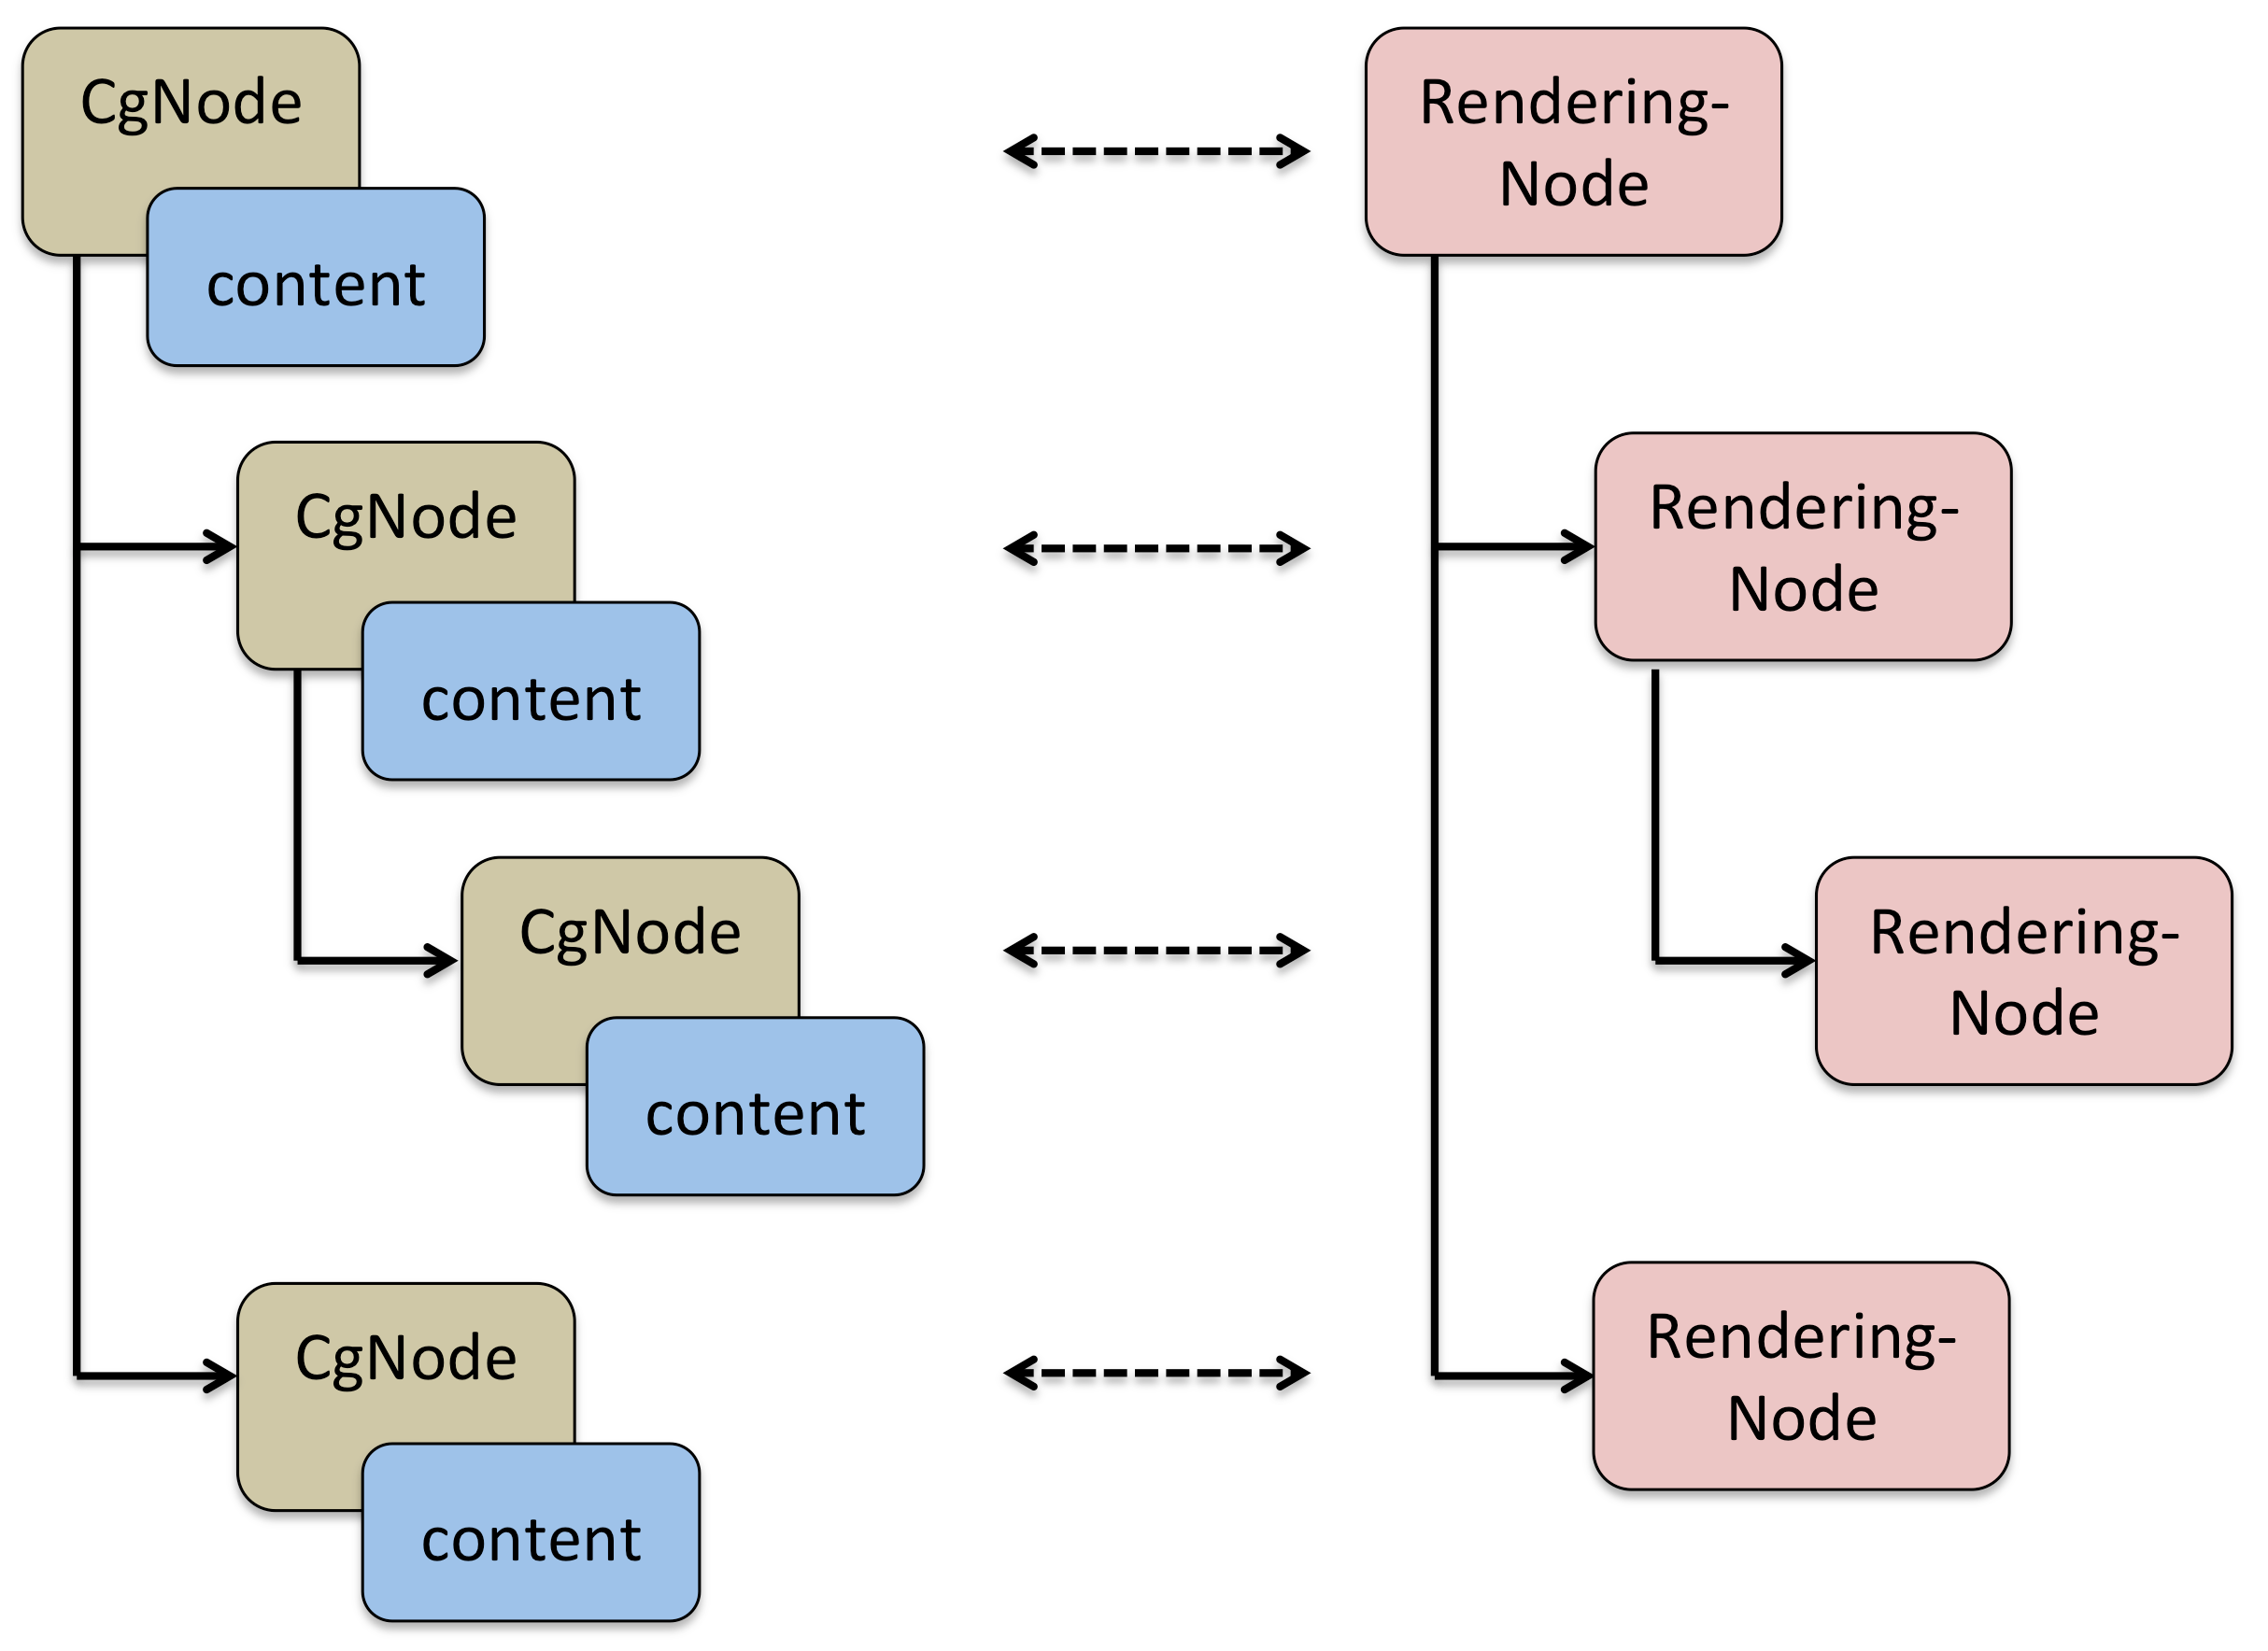
\includegraphics[height=6cm]{images/renderinggraph.png}
\label{fig:renderinggraph.png}
\caption{Zum Szenengraph wird dynamisch ein dualer Renderinggraph aufgebaut. Zu jedem Knoten des Szenengraphen wird ein Renderingknoten im Rendering-System erstellt. Die Renderingknoten �bernehmen die Darstellung der Inhalte.}
\end{figure} 

Jedes Rendering-System stellt einen zentralen Frame zu Verf�gung. Um ein Rendering-System zu verwenden, wir eine Instanz des Frames erzeugt. F�r die Visualisierung von einzelnen Knoten im Szenengraphen gibt es ein Plugin-Konzept. F�r die unterschiedlichen Daten in den Szenengraph-Knoten k�nnen Fabriken registriert werden, die jeweils die zugeh�rigen Renderknoten erzeugen. Es entsteht also ein dualer Szenengraph f�r das Rendering-System. Fabriken implementieren das Interface {\verb IRenderObjectsFactory<T> }. Sie k�nnen dem Rendering-System dann �ber die Methode 
\begin{verbatim} 
public void registerRenderObjectsFactory(IRenderObjectsFactory<T> factory);
\end{verbatim}
des zentralen Frames mitgeteilt werden. Standard-Fabriken werden direkt �ber die Rendering-Systeme registriert. Eigene Fabriken k�nnen auch in den Anwendungsprojekten registriert werden.

\subsubsection{JOGL}
\label{section:JOGL}

\begin{verbatim} 
cgresearch.rendering.jogl
\end{verbatim}

Das Rendering-System JOGL bietet die maximale Freiheit - es wird direkt auf die OpenGL-Ebene zugegriffen.

\subsubsection{jMonkey}
\label{section:jMonkey}

\begin{verbatim} 
cgresearch.rendering.jmonkey
\end{verbatim}

\subsection{Lichtquellen}
\label{sec:lights}

Lichtquellen in der Szene werden zentral �ber den Wurzelknoten verwaltet. Der Wurzelknoten hat dazu einen speziellen Typ, n�mlich \verb+CgRootNode+ und kann aus der zentralen Anwendung, abgeleitet von \verb+CgApplication+, heraus erreicht werden: 
\begin{verbatim}
CgRootNode getCgRootNode()
\end{verbatim}
Der Wurzelknoten bietet Zugriff auf die Anzahl der Lichtquellen (\verb+int getNumberOfLights()+) und auf eine einzelne Lichtquelle (\verb+getLight(int index)+). �ndert sich die Beleuchtungssituation, so werden auch die verwendeten Renderer aktualisiert. Dazu muss die Methode \verb+lightingChanged()+ aufgerufen werden.

Lichtquellen sind in der Klasse \verb+LightSource+ repr�sentiert. Neben Position, Farbe und Richtung (falls ben�tigt) wird dort auch der Typ der Lichtquelle abgelegt. Aktuell sind folgende Typen umgesetzt:
\begin{itemize}
\item Punktlichtquelle
\item Richtungslichtquelle
\item Spot-Lichtquellen
\end{itemize}

Die drei verschiedenen Lichtquellen werden dann im Renderer (Klasse\\ \verb+cgresearch.rendering.jogl.core.JoglRenderer3D+ an OpenGL �bergeben. Dabei wird zur Unterscheidung der drei Typen folgenden Konvention verwendet:
\begin{itemize}
\item Punktlichtquelle: \verb+GL2.GL_SPOT_CUTOFF < 0+ und \verb+GL2.GL_POSITION.w = 1+
\item Richtungslichtquelle: \verb+GL2.GL_SPOT_CUTOFF < 0+ und \verb+GL2.GL_POSITION.w < 1+ (die Richtung steht in \verb+GL2.GL_POSITION+
\item Spot-Lichtquelle: \verb+GL2.GL_SPOT_CUTOFF > 0+, Position steht in \verb+GL2.GL_POSITION+, Richtung steht in \verb+GL2.GL_DIRECTION+
\end{itemize}

Im der Swing Benutzerschnittstelle lassen sich die Lichtquellen verwalten und dynamisch ver�ndern. Den zugeh�rigen Editor findet man im Men� unter \emph{Rendering $\rightarrow$ Light}. Durch Doppelklick auf einen Wert kann dieser ver�ndert werden.

Die Standart-Lichtquellen sind direkt im Konstruktion der Klasse \verb+CgApplication+ gesetzt.

\emph{Achtung: Aktuell sind noch nicht alle Shader umgestellt, um die Lichtquellen der Szene zu verwenden. Manche Shader haben die verwendeten Lichtquellen noch fest im Shadercode verdrahtet.}

Shader, die die Beleuchtung auf Basis der Lichtquellen berechnen:
\begin{itemize}
\item \textbf{Material.SHADER\_PHONG\_SHADING:} Phong Beleuchtungsmodell, Phong Shading Verfahren 
\begin{itemize}
\item VS: \emph{shader/vertex\_shader\_phong\_shading.glsl}
\item FS: \emph{shader/fragment\_shader\_phong\_shading.glsl}
\end{itemize}
\item \textbf{Material.SHADER\_TEXTURE\_PHONG:} Phone Beleuchtungsmodell auf Textur, Phone Shading Verfahren
\begin{itemize}
\item VS:\emph{ shader/vertex\_shader\_texture\_phong\_shading.glsl}
\item FS: \emph{shader/fragment\_shader\_texture\_phong\_shading.glsl}
\end{itemize}
\end{itemize}

\subsection{Texturen und Shader}

Shader und Texturen werden je in einem zentralen Ressourcen-Manager verwaltet. Der Zugriff erfolgt so:
\begin{verbatim}
ResourceManager.getShaderManagerInstance();
\end{verbatim}
und 
\begin{verbatim}
ResourceManager.getTextureManagerInstance();
\end{verbatim}

\subsubsection{Texturen}

Will man beispielsweise eine Textur verwenden, dann vergibt man daf�r eine Id und registriert diese Id und die Textur im zugeh�rigen Ressourcen-Manager:
\begin{verbatim}
CgTexture myTexture = new CgTexture("textures/my_texture.png");
String myTextureId = "myId";
ResourceManager.getTextureManagerInstance().addResource(myTextureId,
				myTexture);
\end{verbatim}

Alternativ kann eine Textur auch direkt aus einem \verb+BufferedImage+ erzeugt werden.

Die Id verwendet man dann im Material, um die Textur zu verwenden, z.B.:
\begin{verbatim}
ITriangleMesh myMesh = new TriangleMesh();
myMesh.getMaterial().setTextureId(myTextureId);
\end{verbatim}

\subsubsection{Shader}

Das Verwenden von Shadern funktioniert analog. Shader werden durch die Klasse \verb+CgGlslShader+ repr�sentiert. Zur Konstruktion eines \verb+CgGlslShader+-Objektes �bergibt man die Dateinamen des Vertex- und des Fragmentshader-Codes.

Es ist m�glich, mehrere Renderdurchg�nge hintereinander durchzuf�hren in denen unterschiedliche Shader verwendet werden. Dazu setzt man mit der Methode
\begin{verbatim}
getMaterial().addShaderId(String shaderId)
\end{verbatim}
einfach mehrere Shader in einem Material.

\subsection{Picking}

\emph{Achtung: Picking wird aktuell nur mit dem JOGL-Rendering-System unterst�tzt.}

Das cg-Framework unterst�tzt ein System zum 'Picking' von Objekten (Punkten) im 3D-Fenster und zum Verschieben dieser Objekte. Es k�nnen allerdings nicht beliebige Szenenobjekte ausgew�hlt werden. Stattdessen werden Picking-Items explizit in die Szene eingef�gt und mit diesen interagiert.

\subsubsection{Erstellen von Picking-Items}

Zum Arbeiten mit Picking-Items muss zun�chst eine Klasse implementiert werden, die von der abstrakten Klasse \verb+CgApplicationPickable+ erbt. Au�erdem m�ssen ein oder mehrere Picking-Items in die Szene eingef�gt werden. Zur Repr�sentation von Picking-Items gibt es die Klasse \verb+PickingItem+. Ein Picking-Item erzeugt mal also beispielsweise mit
\begin{verbatim}
PickingItem item = new PickingItem(VectorMatrixFactory.newIVector3(0,0,0));
\end{verbatim}
Der dem Konstruktor �bergebene Vektor stellt die Position des Picking-Items dar. Um ein Picking-Item in die Szene einzuf�gen, verwendet man die Methode \verb+addPickingItem+ des Objektes, das von \verb+CgApplicationPickable+ erbt. In der 3D-Darstellung wird ein Picking-Item als eine (graue) Kugel dargestellt. Die Gr��e der Kugel muss nat�rlich der Dimension der Szene angepasst werden. Da diese Anpassung nicht automatisch vorgenommen werden kann, muss der Anwender die Einstellung selber vornehmen. Dies geschieht �ber ein Singleton-Objekt \emph{Picking}, dass das Picking verwaltet. Auf dieses Objekt greift man mit \emph{Picking.getInstance()} zu. Die Skalierung wird mit dem Aufruf
\begin{verbatim}
Picking.getInstance().setScaling(0.1);
\end{verbatim}
vorgenommen.

\subsubsection{Interaktion mit Picking-Items}

Picking-Items k�nnen ausgew�hlt und in $x$-, $y$- und $z$-Richtung verschoben werden. Um mit den Picking-Items interagieren zu k�nnen, muss zun�chst in den Picking-Modus gewechselt werden. 

\emph{Achtung: Im Picking-Modus kann die Kamera nicht mehr per Maus gesteuert werden!}

In den Picking-Modus wechselt man, indem man auf das entsprechende Icon in der Schnellstarte-Toolbar auf der linken Seite geklickt wird.
(
\includegraphics[height=0.5cm]{../../assets/icons/picking.png}). Das Icon verf�rbt sich dann in Orange. Befindet man sich im Picking-Modus, dann kann man ein Picking-Item ausw�hlen und verschieben.

\vspace{0.5cm}

\emph{Selektion} Zum Ausw�hlen eines Picking-Items klickt man in der 3D-Szene auf das Item. Ein Item wird dann ausgew�hlt, wenn man ausreichend genau darauf geklickt hat. Befinden sich mehrere Picking-Items in der gleichen Sichtbarkeitslinie, dann wird das ausgew�hlt, das der Kamera am n�chsten liegt. Das ausgew�hlte Picking-Item erkennt man daran, dass es gelb eingef�rbt ist und dass daf�r ein Koordinatensystem gezeichnet wird. Im Koordinatensystem zeigt der rote Pfeil in die $x$-Richtung, der gr�ne Pfeil in die $y$-Richtung und der blaue Pfeil in die $z$-Richtung.

\vspace{0.5cm}

\emph{Verschieben} Das aktuell selektierte Picking-Item kann in $x$-, $y$- und $z$-Richtung verschoben werden. Die Richtungen sind durch die entsprechenden Pfeile angegeben. Zum Verschieben in eine Richtung dr�ckt man die zugeh�rige Taste auf der Tastatur, h�lt die linke Maustaste gedr�ckt und bewegt die Maus nach links bzw. nach rechts. Eine Mausbewegung nach links bewegt das Picking-Item gegen die Pfeilrichtung, eine Mausbewegung nach rechts bewegt das Picking-Item in Pfeilrichtung. Zur Bewegung in die $x$-Richtung dr�ckt man die $x$-Taste, analog $y$ und $z$.

\subsection{Alpha-Blending}

In jeder Szene kann Alpha-Blending (Transparenz) verwendet werden. Zun�chst muss man dazu in dem Szenen-Wurzelknoten \verb+CgRootNode+ Blending aktivieren: 

\begin{verbatim}
getCgRootNode().setUseBlending(true);
\end{verbatim}

F�r jedes Objekt der Szene, das Alpha-Blending verwendet soll, setzt man die Transparenz individuell in dessen Material:

\begin{verbatim}
<Objekt>.getMaterial().setTransparency(0.5);
\end{verbatim}

G�ltig sind alle Werte zwischen 0 (vollst�ndig transparent) und 1 (vollst�ndig opaque).

Um Transparenzen verwenden zu k�nnen, muss das Blending vom verwendeten Shader unterst�tzt werden. Dies ist aktuell f�r die Shader \emph{Phong Shading} und \emph{Textur} der Fall.
\section{Verwendung}
\label{section:verwendung_framework}

In diesem Abschnitt werden einige Anwendungsf�lle f�r das Framework vorgestellt. Es ist aber immer m�glich, dass im Framework Funktionalit�t enthalten ist, die hier noch nicht beschrieben wird. Eine zweite Anlaufstation f�r Anwendungsf�lle sind die Beispielanwendungen im Modul \verb+cgresearch.apps+.

\subsection{Dreiecksnetze}

F�r Dreiecksnetze existiert das Interface \verb+ITriangleMesh+. Ein Dreiecksnetz (hier Kugel mit einer Tesselierung von 10x10 Fl�chen) kann so erzeugt und in den Szenengraphen eingef�gt werden: 
\begin{verbatim}
ITriangleMesh mesh = TriangleMeshFactory.createSphere(10);
CgNode meshNode = new CgNode(mesh, "mesh");
getCgRootNode().addChild(meshNode);
\end{verbatim}
Alternativ k�nnen Dreiecksnetze auch 'von Hand' erzeugt werden:
\begin{verbatim}
ITriangleMesh mesh = new TriangleMesh();
int a = mesh.addVertex(new Vertex(VectorMatrixFactory.newIVector3(1,0,0));
int b = mesh.addVertex(new Vertex(VectorMatrixFactory.newIVector3(0,1,0));
int c = mesh.addVertex(new Vertex(VectorMatrixFactory.newIVector3(0,0,1));
mesh.addTriangle(new Triangle(a,b,c));
\end{verbatim}
Informationen zu den existierenden Importern f�r Dreiecksnetze finden sich im Abschnitt \ref{sec:import}.

\subsection{Punktwolken}

F�r Punktwolken existiert das Interface \verb+IPointCloud+. Eine Punktwolke (hier W�rfelvolumen) kann so erzeugt und in den Szenengraphen eingef�gt werden: 
\begin{verbatim}
IPointCloud pointCloud = PointCloudFactory.createDummyPointCloud();
CgNode pointCloudNode = new CgNode(pointCloud, "point cloud");
getCgRootNode().addChild(pointCloudNode);
\end{verbatim}
Punkt wollen k�nnen au�erdem aus Dreiecksnetzen erzeugt werden. Dazu werden zufallsverteilt Punkte (hier: 5000) auf der Oberfl�che eines Dreiecksnetzes gesampled:
\begin{verbatim}
IPointCloud pointCloud = MeshSampler.sample(mesh, 5000);
\end{verbatim}
Informationen zu den existierenden Importern f�r Punktwolken finden sich im Abschnitt \ref{sec:import}.

\subsection{Kurven}

Es sind verschiedene Kurven implementiert, die als gemeinsames Interface \verb+ICurve+ verwenden. F�r jede Kurve k�nnen dabei Kontrollpunkte definiert und ausgelesen werden und der Funktionswert und die Ableitung f�r beliebige Parameterwerte ausgewertet werden. Aktuell sind folgende Kurventypen implementiert:
\begin{itemize}
	\item Monom
	\item Lagrange
	\item Hermite
	\item Bezier
\end{itemize}

\subsection{Animierte Daten}

Zur Verwendung zeitlich ver�nderlicher Daten gibt es einen \verb+AnimationTimer+. Dieser ist als Singleton umgesetzt und kann folgenderma�en erreicht werden:
\begin{verbatim}
AnimationTimer animationTimer = AnimationTimer.getInstance();
\end{verbatim}
Der Timer verwaltet eine diskrete Zeitleiste mit Startwert (\verb+minValue+), Endwert (\verb+maxValue+) und aktuellem Wert (\verb+value+).

Der Timer kann �ber verschiedene Wege gesteuert werden:
\begin{itemize}
	\item Zeitliste als Slider direkt im GUI
	\item Einstellungen im Men� \verb+Timer+
	\item direkt �ber die Singleton-Instanz
\end{itemize}	
Unterst�tzung f�r den Timer ist im Szenengraph mit dem Szenengraph-Inhalt \verb+Animation+ gegeben:
\begin{verbatim}
CgNode animationNode = new CgNode(new Animation(), "animation");
\end{verbatim}
Dieser Knoten sorgt daf�r, dass von seinen Kindern nur das angezeigt wird, dessen Index mit dem aktuellen Wert des \verb+AnimationTimers+ �bereinstimmt. F�r dynamische Daten erzeugt man also je einen Szenengraph-Knoten pro Zeitschritt und f�gt diese als Kinder einem Szenengraph-Knoten, der einen \verb+Animation+-Inhalt hat, zu.

Der \verb+AnimationTimer+ kann auch dazu 'missbraucht' werden, um verschiedenen Datens�tze schnell sichtbar und unsichtbar  zu schalten. Hat man mehrere Daten, von denen immer nur genau ein Datensatz angezeigt werden soll, dann kann man die Daten als Kinder eines Animationsknotens in den Szenengraph einf�gen. �ber den Zeitleisten-Slider kann immer genau ein Datensatz sichtbar geschaltet werden.

\subsection{Kamera}

Die virtuelle Kamera wird �ber einen Kamera-Controller gesteuert. Aktuell sind folgende Controller implementiert:
\begin{itemize}
\item \verb+InspectionCameraController+
\item \verb+CameraPathController+
\item \verb+FirstPersonCameraPathController+
\item \verb+MovableInspectionCameraPathController+
\end{itemize}

Der Standard-Controller ist der \verb+InspectionCameraController+. 

Der \verb+InspectionCameraController+ eignet sich besonders zum Betrachten eines Objektes oder einer Szene von allen Seiten. Die Steuerung erfolgt �ber die Maus. Bei gedr�ckter linker Maustasten und gleichzeitiger Bewegung der Maus wird die Kamera um den Referenzpunkt der Kamera herum gedreht. Mit gedr�ckter linker Maustaste kann an das Objekt heran- oder wieder herausgezoomt werden.

Der \verb+CameraPathController+ dient dem Abspielen eines gespeicherten Kamerapfades. Der Kamerapfad wird mit Hilfe von Keypoints vorgegeben. Zwischen den Keypoints wird die Position interpoliert. Die Keypoints k�nnen �ber das Menu \emph{Jogl} $\rightarrow$ \emph{Camera} verwaltet werden (Hinzuf�gen und Entfernen von Keypoints). Ist der \verb+CameraPathController+ selektiert, dann wird der Kamerapfad �ber die Zeitleiste des \verb+AnimationTimers+ kontrolliert. Der vollst�ndige Pfad l�uft �ber die gesamte L�nge der Zeitleiste - dar�ber kann also auch die Aufl�sung der Bewegung und die Geschwindigkeit der Kamerabewegung festgelegt werden.

Alle Einstellungen zur Kamera sind im Camera-Singleton abgelegt. Darauf l�sst sich mit 
\begin{verbatim}
	Camera.getInstance()
\end{verbatim}
zugreifen. In der Kamera kann auch der aktuelle Controller gesetzt werden. Alternativ lassen sich die meisten Kameraeinstellungen auch per GUI im Menu unter \emph{Jogl} $\rightarrow$ \emph{Camera} vornehmen.

\subsection{Film-Export}

Es ist m�glich, die 3D-Darstellung zu exportierten. Konkret kann jeder Zeitschritt als ein Einzelbild exportiert werden. Die Einzelbilder k�nnen dann �ber externe Tools zu Videos zusammengestellt werden. Achtung: Der Export der Einzelbilder kostet einige Zeit. Es ist daher ggf. notwendig, den \verb+AnimationTimer+ mit einer geringeren Geschwindigkeit laufen zu lassen, damit auch wirklich von jedem Frame ein Bild exportiert wird. Das Exportieren der Einzelbilder kann �ber das Menu \emph{Jogl} $\rightarrow$ \emph{Movie Export} gestartet und wieder beendet werden. Dort l�sst sich auch der Ausgabepfad festlegen.

\subsection{Octree}

Zur effizienten Bearbeitung von Szenen eignen sich oft hierarchische Datenstrukturen. Im Framework sind dazu bislang Octrees umgesetzt. Die Octrees sind generisch und wissen zun�chst nicht, welche Daten sie verwalten. Zum Aufbauen eines Octrees ben�tigt man daher ein Objekt, dass mit den konkreten Daten umgeht. Hier ist dies mit den Strategy-Entwurfsmuster umgesetzt. Ein Strategie-Objekt wird verwendet, um eine Factory (Fabrik) zu erzeugen, die den Octree aufbaut. Es existieren aktuell Strategien f�r Dreickecksnetze und Punktwolken. Einen Octree f�r ein Dreiecksnetz erzeugt man so (maximale Tiefe des Baumes 7 und Teilungsgr��e einer Zelle 20):
\begin{verbatim}
OctreeFactoryStrategyTriangleMesh octreeFactoryStrategyMesh = 
 	 	new OctreeFactoryStrategyTriangleMesh(mesh);
OctreeFactory<Integer> octreeFactoryMesh = 
 	 	new OctreeFactory<Integer>(octreeFactoryStrategyMesh);
OctreeNode<Integer> octreeMeshRoot = octreeFactoryMesh.create(7, 20);
\end{verbatim}

\subsection{Daten-Im- und Export}
\label{sec:import}

F�r verschiedenen Datentypen wird der Im- und Export unterst�tzt:

\subsubsection{Dreiecksnetze}

\begin{itemize}
	\item OBJ-Import: Klasse \verb+ObjFileReader+
	\item OBJ-Export: Klasse \verb+ObjFileWriter+
	\item PLY-Import: Klasse \verb+PlyFileReader+
\end{itemize}

Beispielhafter Import aus Obj-Datei:
\begin{verbatim}
ObjFileReader reader = new ObjFileReader();
CgNode meshNode = reader.readFile("meshes/bunny.obj");
\end{verbatim}
Das Ergebnis ist eine \verb+CgNode+, die importierten Meshes aus der Obj-Datei sind als Kindknoten dieses Knotens abgelegt.

 \subsubsection{Motion-Capture-Daten}

\begin{itemize}
	\item Daten aus dem HAW Wellefeldsynthese-Labor: Klasse \verb+MoCapImporter+
\end{itemize}

 \subsubsection{Punktwolken}

\begin{itemize}
	\item ASCII-Daten-Import: Klasse \verb+AsciiPointsReader+
	\item ASCII-Daten-Export: Klasse \verb+AsciiPointsWriter+
\end{itemize}

Beim Import von ASCII-Daten gibt es verschiedene Formate in denen die Punktinformationen vorliegen k�nnen. Um diese mit einem Importer abdecken zu k�nnen, muss beim Import das Format mit angegeben werden. Das Format wird �ber ein Objekt der Klasse \verb+AsciiPointFormat+ repr�sentiert. Es wird davon ausgegangen, dass die Ascii-Daten zeilenweise mit einem konstanten Trennungszeichen angegeben sind. Alle Zeilen, die das Format erf�llen, werden importiert. Um beispielsweise Daten im Format \newline
$<$Position-X$>$ $<$Position-Y$>$ $<$Position-Z$>$ $<$Normale-X$>$ $<$Normale-Y$>$ $<$Normale-Z$>$ \newline
mit einem Leerzeichen als Trennungszeichen einzulesen, wird folgendes Formatierungsobjekt erzeugt:
\begin{verbatim}
AsciiPointFormat format = new AsciiPointFormat()
 	 	.setPosition(0, 1, 2).setNormal(3, 4, 5).setSeparator("\\s+");
\end{verbatim} 
Die Parameter geben die Position des entsprechenden Wertes in der Datenzeile an. Der Konstruktor erzeugt ein Objekt und mit den Methoden wird das Objekt angepasst und jeweils wieder zur�ckgegeben (method chaining). Damit ist es m�glich, das Objekt mit einem Ausdruck zu erzeugen. Au�erdem k�nnen Farbinformation (RGB) und eine Skalierung der Farbwerte angegeben werden.

Der Export arbeitet analog.
\section{Projekte}
\label{section:Projekte}

\subsection{3D Scanner}
\label{section:3dScanner}

\subsubsection{Abh�ngigkeiten}

\begin{itemize}
	\item cg
	\item JOGL
	\item Tinkerforge-Bibliotheken (Unterverzeichnis lib)
\end{itemize}

\subsubsection{Installation}

Zun�chst m�ssen die Projekte cg (Abschnitt \ref{section:cg}) und JOGL (Abschnitt \ref{section:JOGL}) eingerichtet werden. und das Git-Repository (\emph{git.informatik.haw-hamburg.de/srv/git/computergrafik/cg\_3dscanner})  gecloned werden (siehe Abschnitt \ref{section:clone}). Dann wird auch das Projekt \emph{3dscanner} in Eclipse importiert. Als Compiler und f�r die Laufzeitbibliothek muss wegen der Abh�ngigkeit von JOGL Java 1.6 verwendet werden.

Setzen Sie die notwendigen Ressourcenpfade wie unter \ref{section:ressourcen} beschrieben.

\subsubsection{Einrichten des USB-Seriell-Adapters}

Der Treiber (Beispiel Windows XP) befindet sich im Projektverzeichnis unter\newline
\emph{software/software/usb\_rs232/Usb\_to\_Rs232\_2303\_includ\_2\_IC/win98\_winme\_vista\_win2000\_winxp}.\newline
Unter Windows wird die Hardware beim Einstecken automatisch erkannt. Der Treiber kann direkt �ber den Hardware-Wizard installiert werden. Es muss nur das Verzeichnis angegeben werden.

Abbildung \ref{fig:usbserialadapter} beschreibt, wie �berpr�ft wird, ob korrekt ein COM-Port angelegt wurde. Achtung, je nach Betriebssystem, kann es sein, dass beim Neustart eines Rechners ein anderer COM-Port vergeben wird.

\begin{figure}[ht]
\centering

	\subfigure[]{
		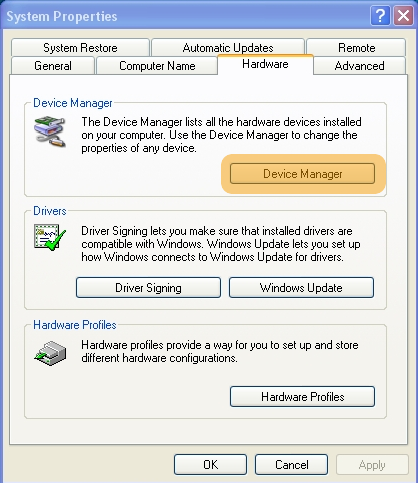
\includegraphics[height=4cm]{images/distance_sensor01.png}
		\label{fig:distance_sensor01.png}
 	}
	\subfigure[]{
		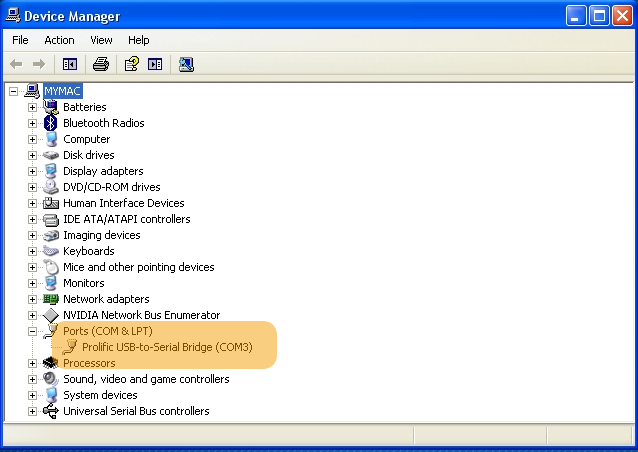
\includegraphics[height=4cm]{images/distance_sensor02.png}
		
 	}
	\caption{Pr�fung, ob nach der Treiberinstallation ein neuer COM-Port angelegt wurde. a) Systemeinstellungsmenu unter Windows, �ffnen des \emph{Device Managers}. b) Es sollte sich ein COM-Port unter dem Men�punkt \emph{Ports (COM\&LPT)} befinden.}
	\label{fig:usbserialadapter}
\end{figure} 

\subsubsection{Testen des Distanzsensors}

Die Software zum Testen des Distanzsensors befindet sich im  Projektverzeichnis um Unterverzeichnis \emph{software/laser\_distance\_sensor}. Die Installation wird �ber \emph{setup.exe} gestartet.

Abbildung \ref{fig:distancesensortest} zeigt, wie die mitgelieferte Software verwendet werden kann, um den Distanzsensor zu testen.

\begin{figure}[ht]
\centering
\subfigure[]{
		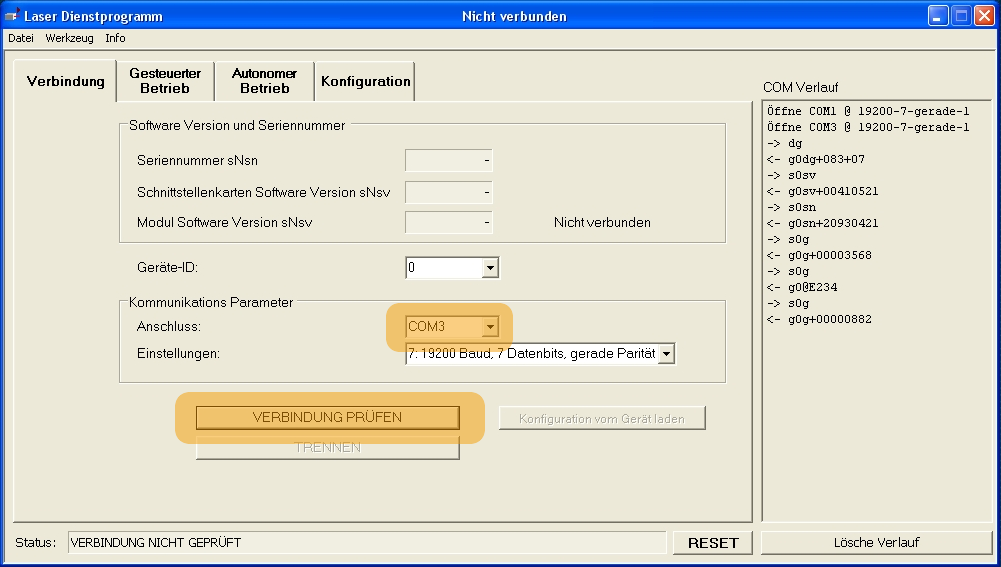
\includegraphics[height=4cm]{images/distance_sensor03.png}
 	}
	\subfigure[]{
		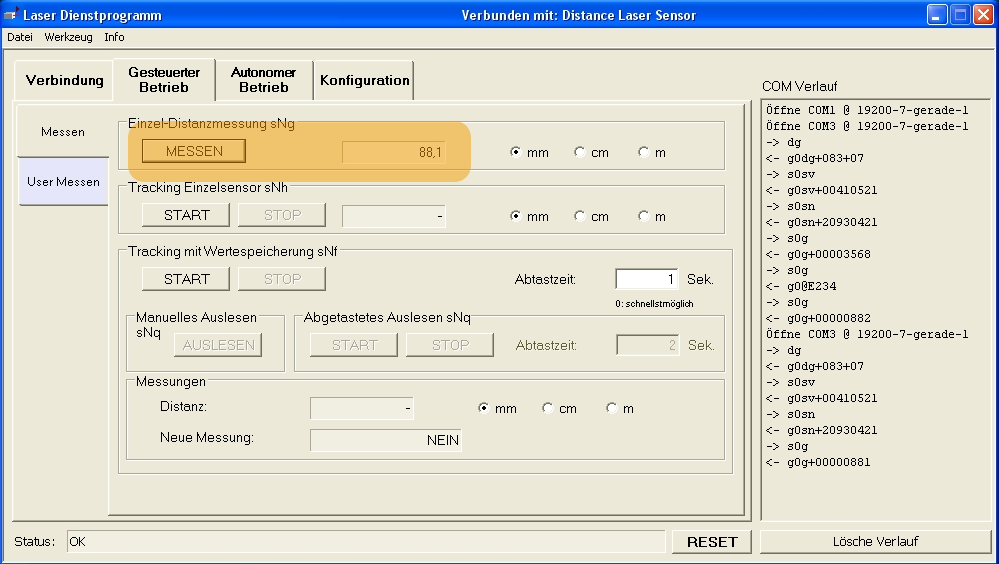
\includegraphics[height=4cm]{images/distance_sensor04.png}
 	}
	\caption{Ausf�hren der installierten Software. a) Auswahl des korrekten COM-Ports und Pr�fen der Verbindung (dabei wird die Verbindung aufgebaut). b) Ausf�hren einer Entfernungsmessung, der gemessene Distanzwert wird direkt angezeigt.}
	\label{fig:distancesensortest}
\end{figure} 



\subsection{Urban Reconstruction}
\label{section:urbanreconstruction}

\subsubsection{Abh�ngigkeiten}

\begin{itemize}
	\item cg
	\item JOGL
\end{itemize}

\subsubsection{Installation}

Zun�chst m�ssen die Projekte cg (Abschnitt \ref{section:cg}) und JOGL (Abschnitt \ref{section:JOGL}) eingerichtet werden. und das Git-Repository (\emph{git.informatik.haw-hamburg.de/srv/git/computergrafik/cg\_urbanreconstruction})  gecloned werden (siehe Abschnitt \ref{section:clone}). Dann wird auch das Projekt \emph{3dscanner} in Eclipse importiert. Als Compiler und f�r die Laufzeitbibliothek muss wegen der Abh�ngigkeit von JOGL Java 1.6 verwendet werden.

Setzen Sie die notwendigen Ressourcenpfade wie unter \ref{section:ressourcen} beschrieben.
%\section{Best Practises}

\subsection{Git}

\subsubsection{Anlegen eines neuen lokalen Repositories}

\begin{itemize}
	\item mkdir $<$Verzeichnisname$>$
	\item cd $<$Verzeichnisname$>$
	\item git init
\end{itemize}

\subsubsection{Anlegen eines neuen Repositories auf dem Server}

\begin{itemize}
	\item mkdir $<$Verzeichnisname$>$
	\item cd $<$Verzeichnisname$>$
	\item git init --bare
\end{itemize}

Beispiel:

\begin{itemize}
	\item mkdir cg
	\item cd cg
	\item git init --bare
\end{itemize}

\subsubsection{Setzen eines Remote Repositories}

\begin{itemize}
	\item git remote add $<$Name des Remote Repositories$>$ $<$Pfad zum Repository$>$
	\item Beispiel (gleicher Rechner): git remote add local /Users/abo781/repository/cg
	\item Beispiel (Server): git remote add server ssh://abo781@git.informatik.haw-hamburg.de/srv/git/computergrafik/cg
\end{itemize}

\subsubsection{Lokale �nderungen an Server Repository senden}

\begin{itemize}
	\item git push $<$Name des Remote Repositories$>$ $<$Name des Branches$>$
	\item Beispiel: git push server master
\end{itemize}

\subsubsection{Lokales Klon-Repository von Server holen}
\label{section:clone}

\begin{itemize}
	\item git clone $<$Name des Remote Repositories$>$ 
	\item Beispiel: git clone ssh://abo781@git.informatik.haw-hamburg.de/srv/git/computergrafik/cg
\end{itemize}

\subsection{Sonar}

Starten von Sonar mit
\begin{verbatim}
cd <Sonar-Verzeichnis>/bin/<Betriebssystem>/
./sonar.sh start
\end{verbatim}

Pr�fen, ob der Sonar-Server l�uft (Im Browser):
\begin{verbatim}
http://localhost:9000/
\end{verbatim}

Sonar-Analyse durchf�hren (ben�tigt Maven-Installation).
\begin{verbatim}
mvn sonar:sonar
\end{verbatim}

\end{document}